% !TEX program = xelatex
%
% 实验一：目标检测与识别 —— 报告模板（基于 YOLOv8 的桌面杯鼠双类检测）
%
% 编译：xelatex report.tex（连编两次生成目录/页码）
%       - 本地 TeX Live / MacTeX：直接 xelatex
%       - Overleaf：编译器选 XeLaTeX 后上传整个 report/ 目录即可
%
% 使用前请修改：
%   1) 封面「个人信息」中的姓名 / 学号 / 班级 / 指导教师 / 日期
%   2) 第 2 节「实验环境」表格中与实际一致的部分
%   3) 图表由 scripts/gen_report_assets.py 自动生成（改了数据重新跑一遍即可）
%
\documentclass[UTF8,a4paper,zihao=-4]{ctexart}

% ============================== 宏包 ==============================
\usepackage{geometry}        % 页边距
\usepackage{graphicx}        % 插图
\usepackage{booktabs}        % 三线表
\usepackage{longtable}       % 跨页表
\usepackage{array}
\usepackage{amsmath,amssymb}
\usepackage{caption}
\usepackage{subcaption}      % 子图
\usepackage{xcolor}
\usepackage{listings}        % 代码块
\usepackage{fancyvrb}        % 原文输入 git 记录
\usepackage{tikz}            % 架构图
\usetikzlibrary{positioning,arrows.meta}
\usepackage{hyperref}
\usepackage{underscore}        % 允许正文直接书写下划线（URL 含 _，如 Roboflow 链接）
\usepackage{xurl}              % \url 可在任意字符处断行，长 URL 不溢出

\geometry{top=2.6cm,bottom=2.6cm,left=2.8cm,right=2.8cm}
\graphicspath{{figures/}}    % 图片目录：report/figures/

\hypersetup{
  colorlinks=true, linkcolor=blue, urlcolor=blue, citecolor=blue,
  bookmarksnumbered=true, pdfstartview=FitH,
  pdftitle={实验一：目标检测与识别},
  pdfauthor={马晨曦},
}

\captionsetup{font=small}
\setlength{\parskip}{0.3em}

% 代码块样式（注释保持英文，避免 CJK 等宽字体问题）
\lstdefinestyle{code}{
  basicstyle=\ttfamily\small, frame=single, breaklines=true,
  columns=flexible, tabsize=2, numbers=left, numberstyle=\tiny\color{gray},
  backgroundcolor=\color{gray!6}, xleftmargin=1.5em, framexleftmargin=1.5em,
}

% ============================== 封面 ==============================
\begin{document}

\thispagestyle{empty}
\begin{center}
  \vspace*{1.2cm}
  {\zihao{2}\heiti 实验一：目标检测与识别}\\[0.4cm]
  {\zihao{4}\songti —— 基于 YOLOv8 的桌面杯鼠双类检测与 ROS2 实时发布 ——}\\[2.2cm]

  \renewcommand{\arraystretch}{1.8}
  \zihao{4}
  \begin{tabular}{r@{\hspace{0.8em}}l}
    课程名称 & \underline{\makebox[10em]{计算机视觉}} \\[0.4em]
    实验名称 & \underline{\makebox[10em]{实验一}} \\[0.4em]
    姓\qquad 名 & \underline{\makebox[10em]{马晨曦}} \\[0.4em]
    学\qquad 号 & \underline{\makebox[10em]{24020036047}} \\[0.4em]
    班\qquad 级 & \underline{\makebox[10em]{中外合作办学2班}} \\[0.4em]
    指导教师 & \underline{\makebox[10em]{}} \\[0.4em]
    完成日期 & \underline{\makebox[10em]{2026 年 8 月}} \\[0.4em]
  \end{tabular}
\end{center}
\clearpage

% ============================== 摘要 ==============================
\begin{abstract}
  本实验以桌面上的\emph{杯子（cup）}与\emph{鼠标（mouse）}两类物体为目标，
  实现基于 YOLOv8 的实时目标检测与识别，并部署到 Jetson Orin NX 嵌入式平台、
  通过 ROS2 发布识别结果。针对原始数据集严重类别不平衡（鼠标样本不足）的问题，
  引入 Roboflow 公开数据补充训练并构造 1500:1110 的平衡数据集，采用 COCO 预训练
  权重迁移学习微调双类模型。训练在云端 RTX 5090 上约 70 分钟完成，验证集
  mAP50 达 0.975；在自采集的 20 张个人测试集上，杯子 100\%、鼠标 90\%、
  总体 95\%，满足验收要求（$\geq 80\%$）。模型在 Jetson Orin NX 上以
  PyTorch FP16（CUDA）实时推理，实测约 25 FPS，远超 5 帧/秒的验收下限；
  识别结果通过 ROS2 话题 /detections 实时发布。最后对典型错误案例进行了分析并给出改进方向。

  \vspace{0.6em}
  \noindent\textbf{关键词}：目标检测；YOLOv8；迁移学习；Jetson；FP16 推理；ROS2
\end{abstract}

\tableofcontents
\clearpage

% ============================== 正文 ==============================
\section{实验目的与要求}
\subsection{实验目的}
\par 掌握基于深度学习的通用目标检测方法，熟悉从\emph{数据采集、标注、训练、评估到
嵌入式部署}的完整流程；能够针对实际场景解决类别不平衡、领域差异等工程问题，并具备
模型部署与实时推理的工程能力。

\subsection{实验要求}
\begin{itemize}
  \item 同时识别 \textbf{2 类及以上}桌面物体（本实验：杯子、鼠标）；
  \item 采用 \textbf{YOLOv8} 框架训练模型，可使用公开数据\emph{补充训练}；
  \item 自行采集并标注数据，\textbf{测试集必须使用个人数据}；
  \item 在 \textbf{Jetson Orin NX} 上实时运行，帧率 $\geq 5$ FPS，实时显示
        类别、检测框与置信度；
  \item 通过 \textbf{ROS2} 发布识别结果；
  \item 对 20 个物体进行测试，正确率 $\geq 80\%$，保存测试结果与典型错误案例；
  \item 代码与结果上传个人 GitHub，按增量提交，禁止单次全量提交。
\end{itemize}

\section{实验环境}
\begin{table}[htbp]
  \centering
  \caption{实验环境与软件栈}
  \begin{tabular}{p{2.2cm} p{3.8cm} p{7.6cm}}
    \toprule
    阶段 & 硬件 / 系统 & 关键软件 \\
    \midrule
    数据准备 & 个人电脑 / macOS & Roboflow 公开数据、自研构建脚本 \\
    训练（本地） & Mac（Apple 芯片）/ macOS & Python 3.x、torch 2.13.0（MPS）、
      ultralytics 8.4.127 \\
    训练（云端） & AutoDL RTX 5090（32 GB）/ Ubuntu & torch 2.12.1+cu130、CUDA 13.0、
      ultralytics 8.4.127 \\
    评估 & 个人电脑 / macOS & OpenCV、自研 evaluate.py \\
    部署 & Jetson Orin NX / JetPack 6.x & PyTorch FP16（CUDA）、OpenCV、
      ROS2（Humble） \\
    \bottomrule
  \end{tabular}
\end{table}

\section{数据集与标注}
\subsection{数据来源与构成}
训练使用公开数据补充、平衡策略如下：
\begin{itemize}
  \item \textbf{杯子（class 0）}：Roboflow 公开杯子数据集
    \texttt{cup-detection} v3（CC BY 4.0），抽取后取 1500 张；
    来源 \url{https://universe.roboflow.com/my-workspace-7j2fi/cup-detection-w8kfb/dataset/3}；
  \item \textbf{鼠标（class 1）}：Roboflow Computer-Mouse 数据集 v2
    （CC BY 4.0，653 项目、1110 张），来源
    \url{https://universe.roboflow.com/machine-learning-chipg/computer-mouse-tqzgh/dataset/2}，
    将其中 \texttt{black-mouse}/\texttt{white-mouse} 子类统一重映射为鼠标类；
  \item \textbf{个人测试集}：自采集并标注 20 张（杯子 10 张 + 鼠标 10 张），
    \emph{不参与训练}，仅用于最终验收测试。
\end{itemize}
平衡后数据集共 2610 张（1500 cup : 1110 mouse），实例级共 3428 个
（cup 2310 : mouse 1118）；按 85:15 分层划分，\texttt{train} 2219 张
（cup 1939 / mouse 952 实例）、\texttt{val} 391 张（cup 371 / mouse 166 实例）。
构建时重建输出目录、随机种子固定，避免训练/验证交叉重复造成数据泄漏。

\begin{figure}[htbp]
  \centering
  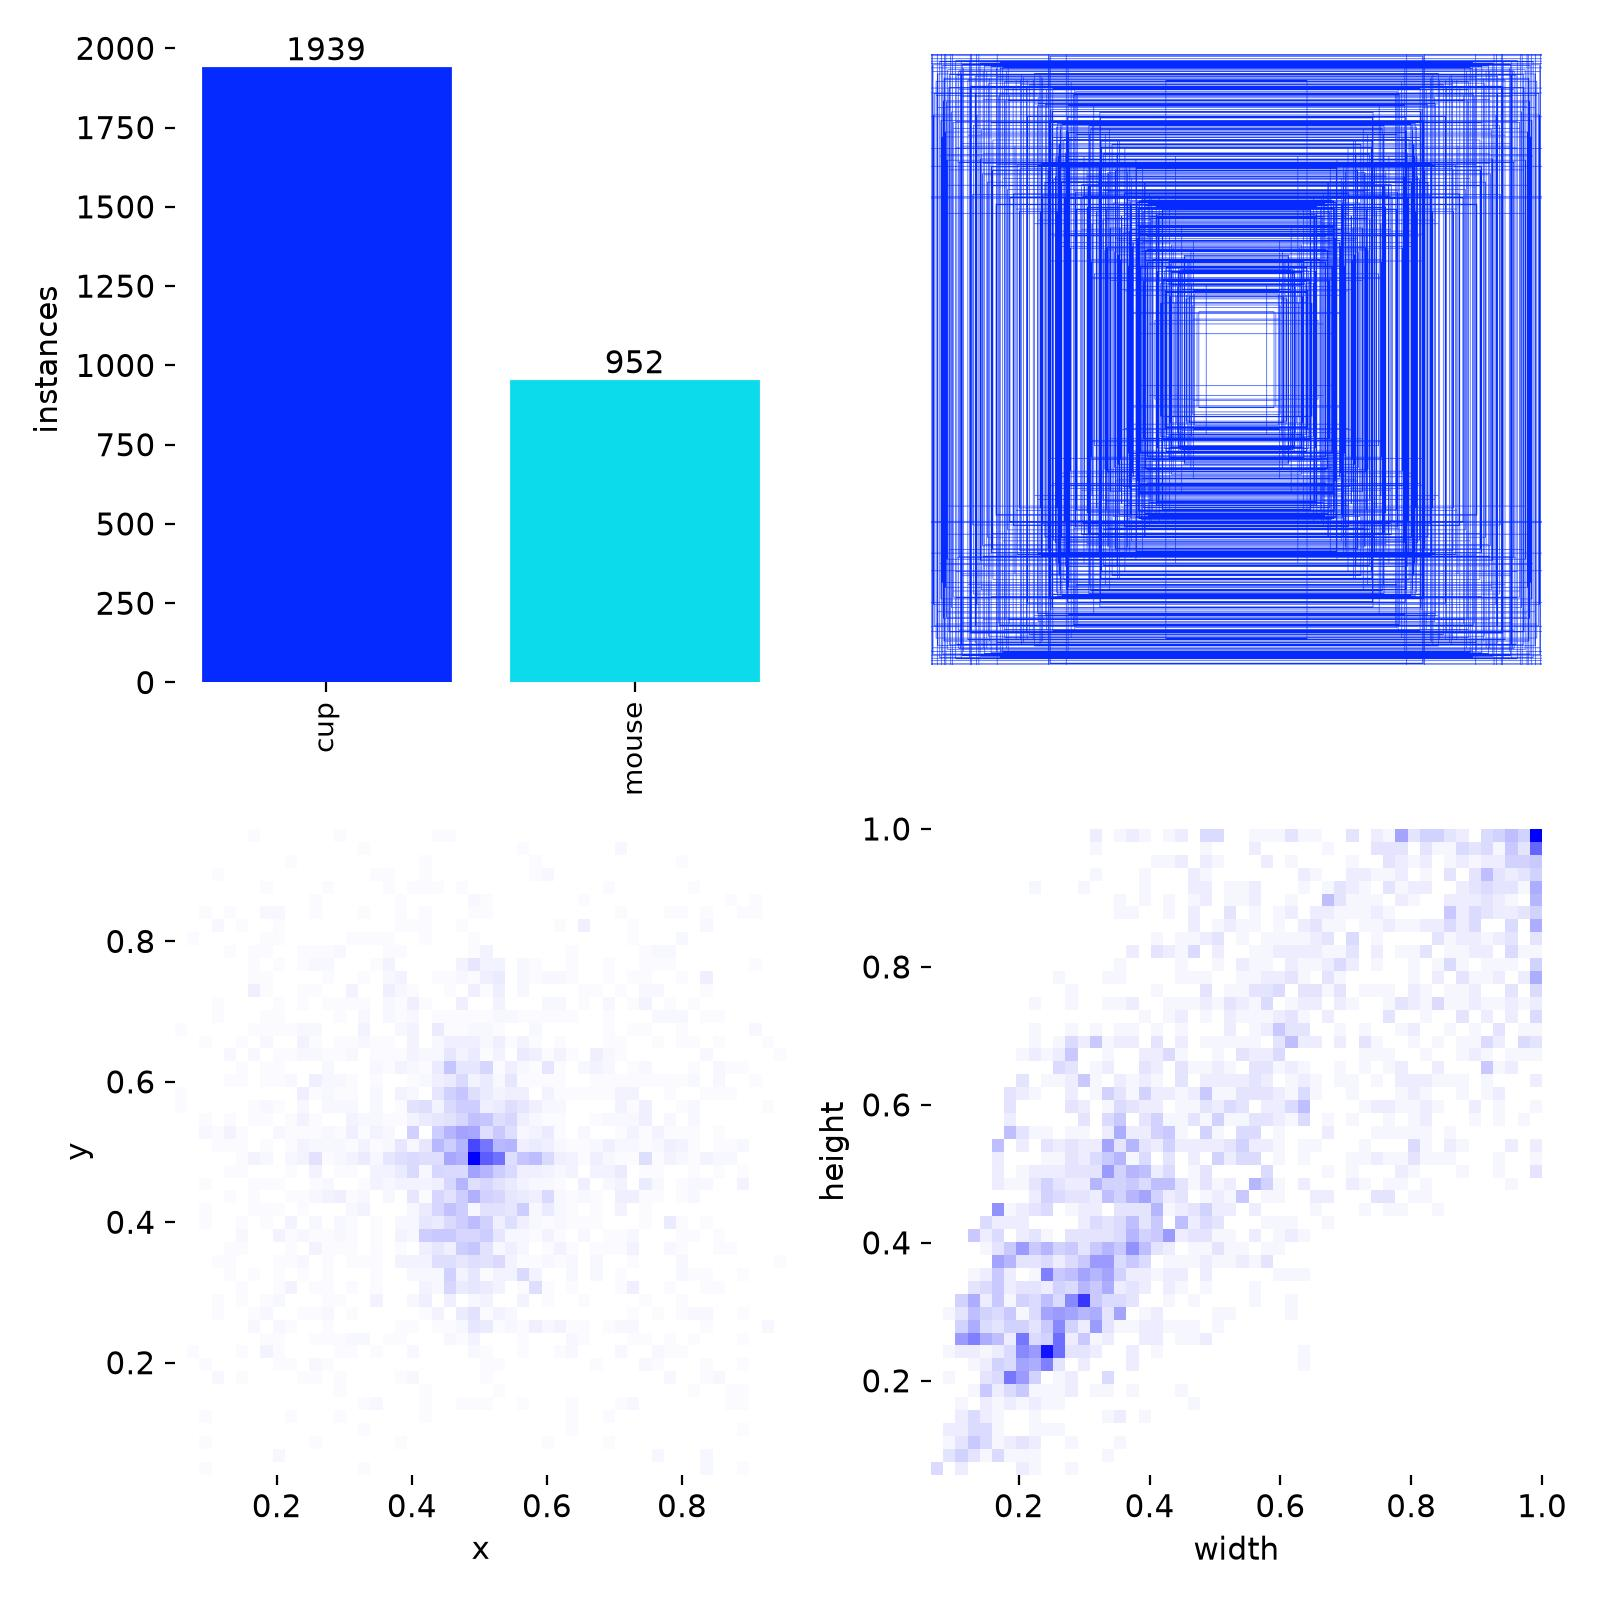
\includegraphics[width=0.85\textwidth,keepaspectratio]{labels_distribution.jpg}
  \caption{训练数据标注分布：左列为标注框在图像中的分布，右列为尺寸与长宽比分布}
\end{figure}

\subsection{标注格式}
采用 YOLO 格式标注：每行 \texttt{class cx cy w h}，其中 \texttt{cx cy}
为归一化中心坐标、\texttt{w h} 为归一化宽高。类别编号映射见表。

\begin{table}[htbp]
  \centering
  \caption{类别映射}
  \begin{tabular}{c l}
    \toprule
    类别编号 & 含义 \\
    \midrule
    0 & cup（杯子） \\
    1 & mouse（鼠标） \\
    \bottomrule
  \end{tabular}
\end{table}

\section{模型与训练方法}
\subsection{YOLOv8 与迁移学习}
YOLOv8 采用 CSPDarknet 骨干与 anchor-free 检测头，包含 C2f 模块与解耦分类/回归头，
在精度与速度间取得良好平衡。本实验加载 COCO 预训练权重 \texttt{yolov8s.pt}
（80 类），将输出类别重映射为 2 类（\texttt{nc=2}）进行迁移学习微调，以加快收敛
并缓解小数据集过拟合。

\subsection{训练超参数}
\begin{table}[htbp]
  \centering
  \caption{训练超参数（截选自 runs/detect/combined\_model\_v3/args.yaml）}
  \begin{tabular}{l l l l}
    \toprule
    参数 & 取值 & 参数 & 取值 \\
    \midrule
    预训练权重 & yolov8s.pt (COCO) & 输入尺寸 & 640$\times$640 \\
    训练轮数 & 150 & batch size & 16 \\
    优化器 & AdamW（auto） & 初始学习率 lr0 & 0.01 \\
    学习率调度 & 余弦退火 cos\_lr & 学习率下限 lrf & 0.01 \\
    动量 / 权重衰减 & 0.937 / 5$\times10^{-4}$ & warmup & 3 epochs \\
    AMP 混合精度 & 开 & 早停 patience & 30 \\
    数据增强 & Mosaic/HSV/缩放/翻转 & close\_mosaic & 末 10 轮 \\
    随机种子 & 0 & 类别重映射 & 开（nc: 80$\to$2） \\
    \bottomrule
  \end{tabular}
\end{table}

\subsection{训练过程}
训练在云端 RTX 5090 上完成，约 27 秒/轮、全程约 70 分钟（本地 Mac MPS 约
5 分钟/轮、预计 12 小时以上）。损失曲线与指标收敛曲线见图。

\begin{figure}[htbp]
  \centering
  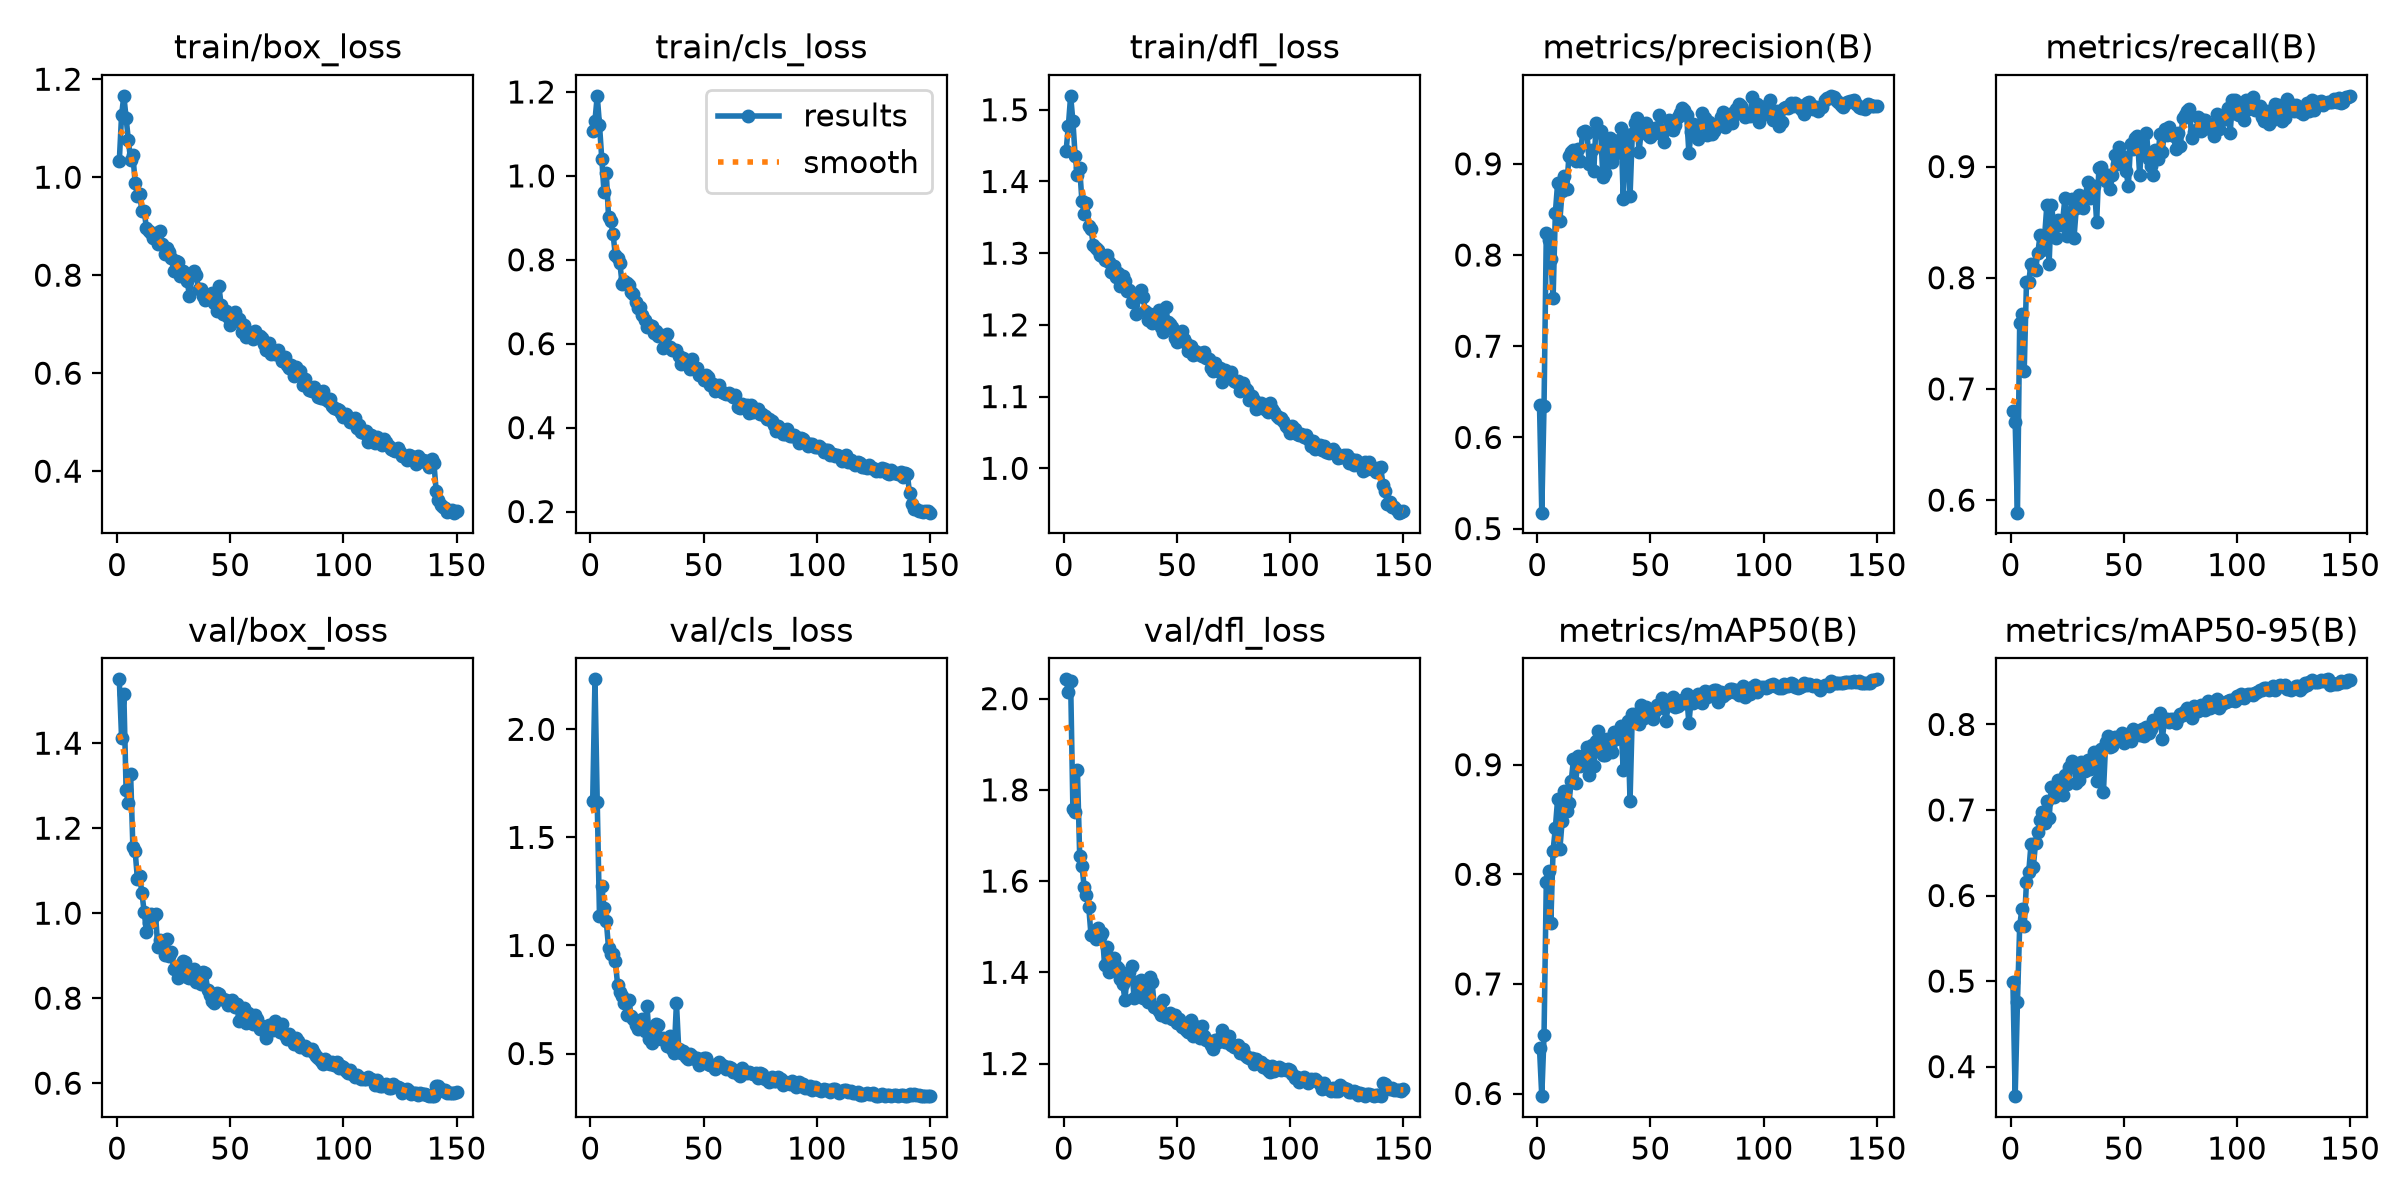
\includegraphics[width=0.9\textwidth,keepaspectratio]{train_curves.png}
  \caption{训练过程曲线：box/cls/dfl 损失随轮次下降，mAP 随轮次上升}
\end{figure}

\begin{figure}[htbp]
  \centering
  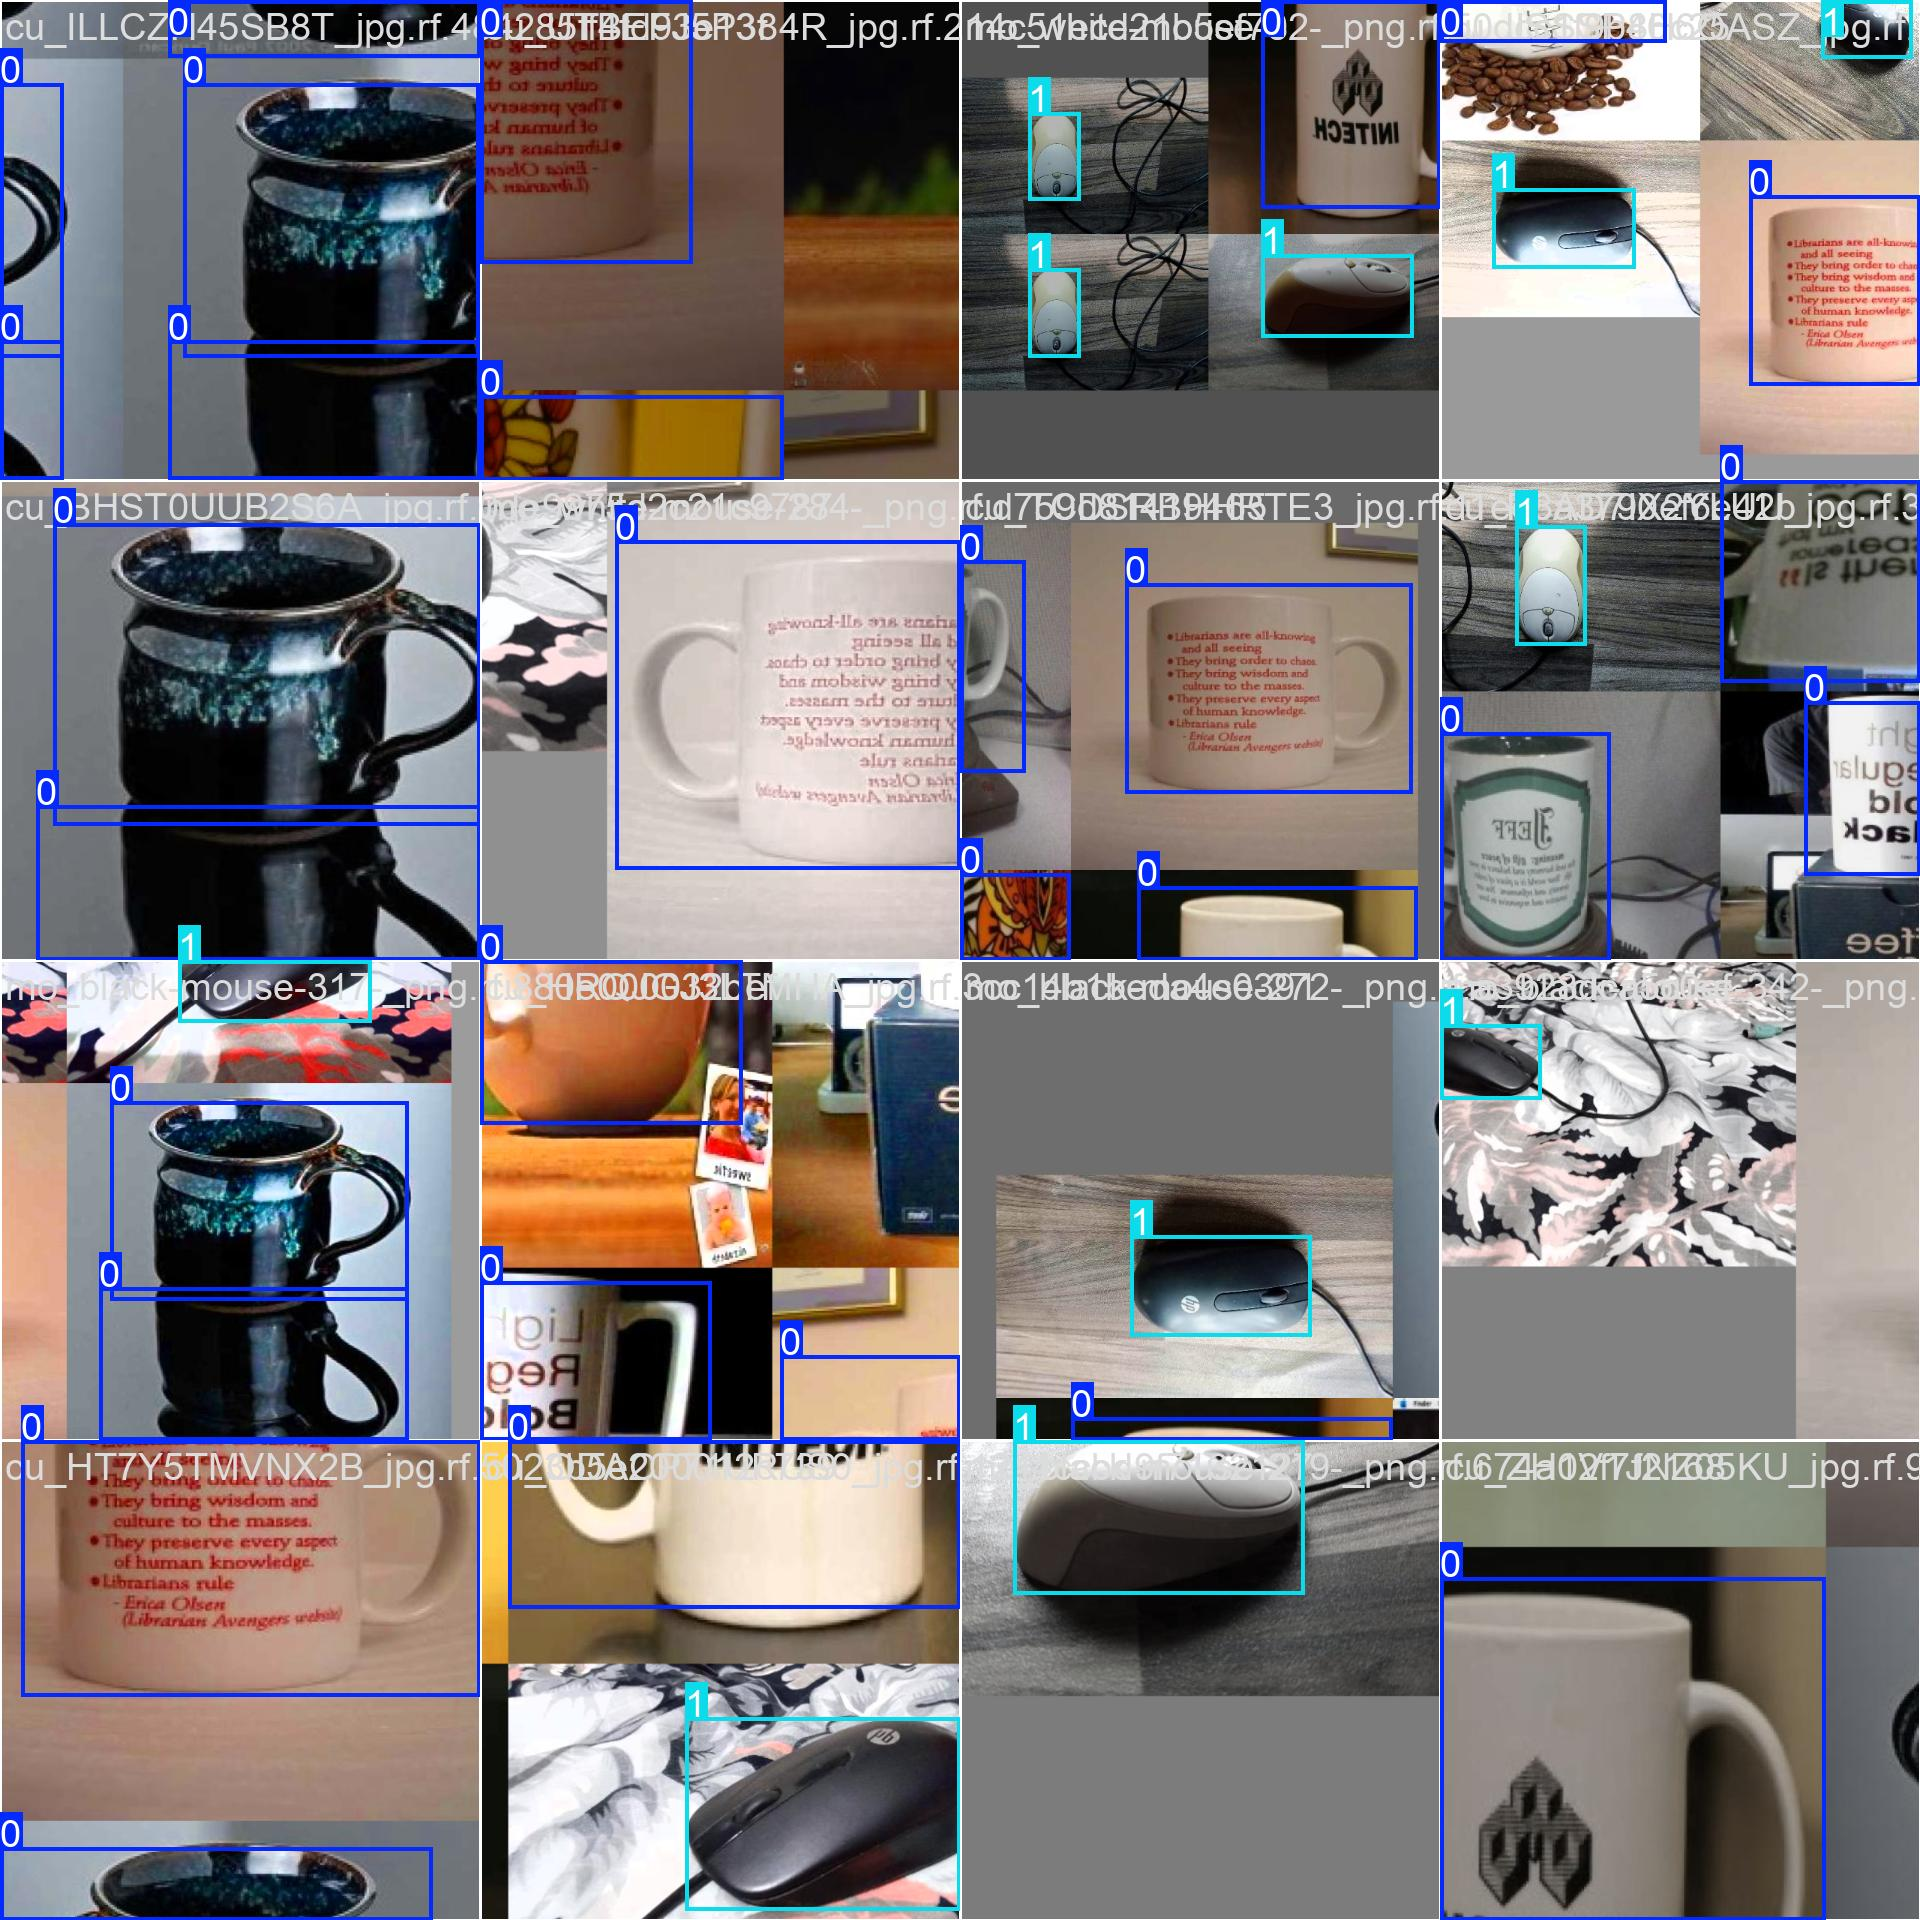
\includegraphics[width=0.9\textwidth,keepaspectratio]{train_batch.jpg}
  \caption{训练批次增强样例（Mosaic 拼接 + HSV/几何变换）}
\end{figure}

\section{实验结果与分析}
\subsection{验证集指标}
验证集 mAP50 收敛至 \textbf{0.975}（best 权重，第 150 轮）。PR 曲线、F1 曲线与
归一化混淆矩阵见图。

\begin{figure}[htbp]
  \centering
  \begin{subfigure}[b]{0.45\textwidth}
    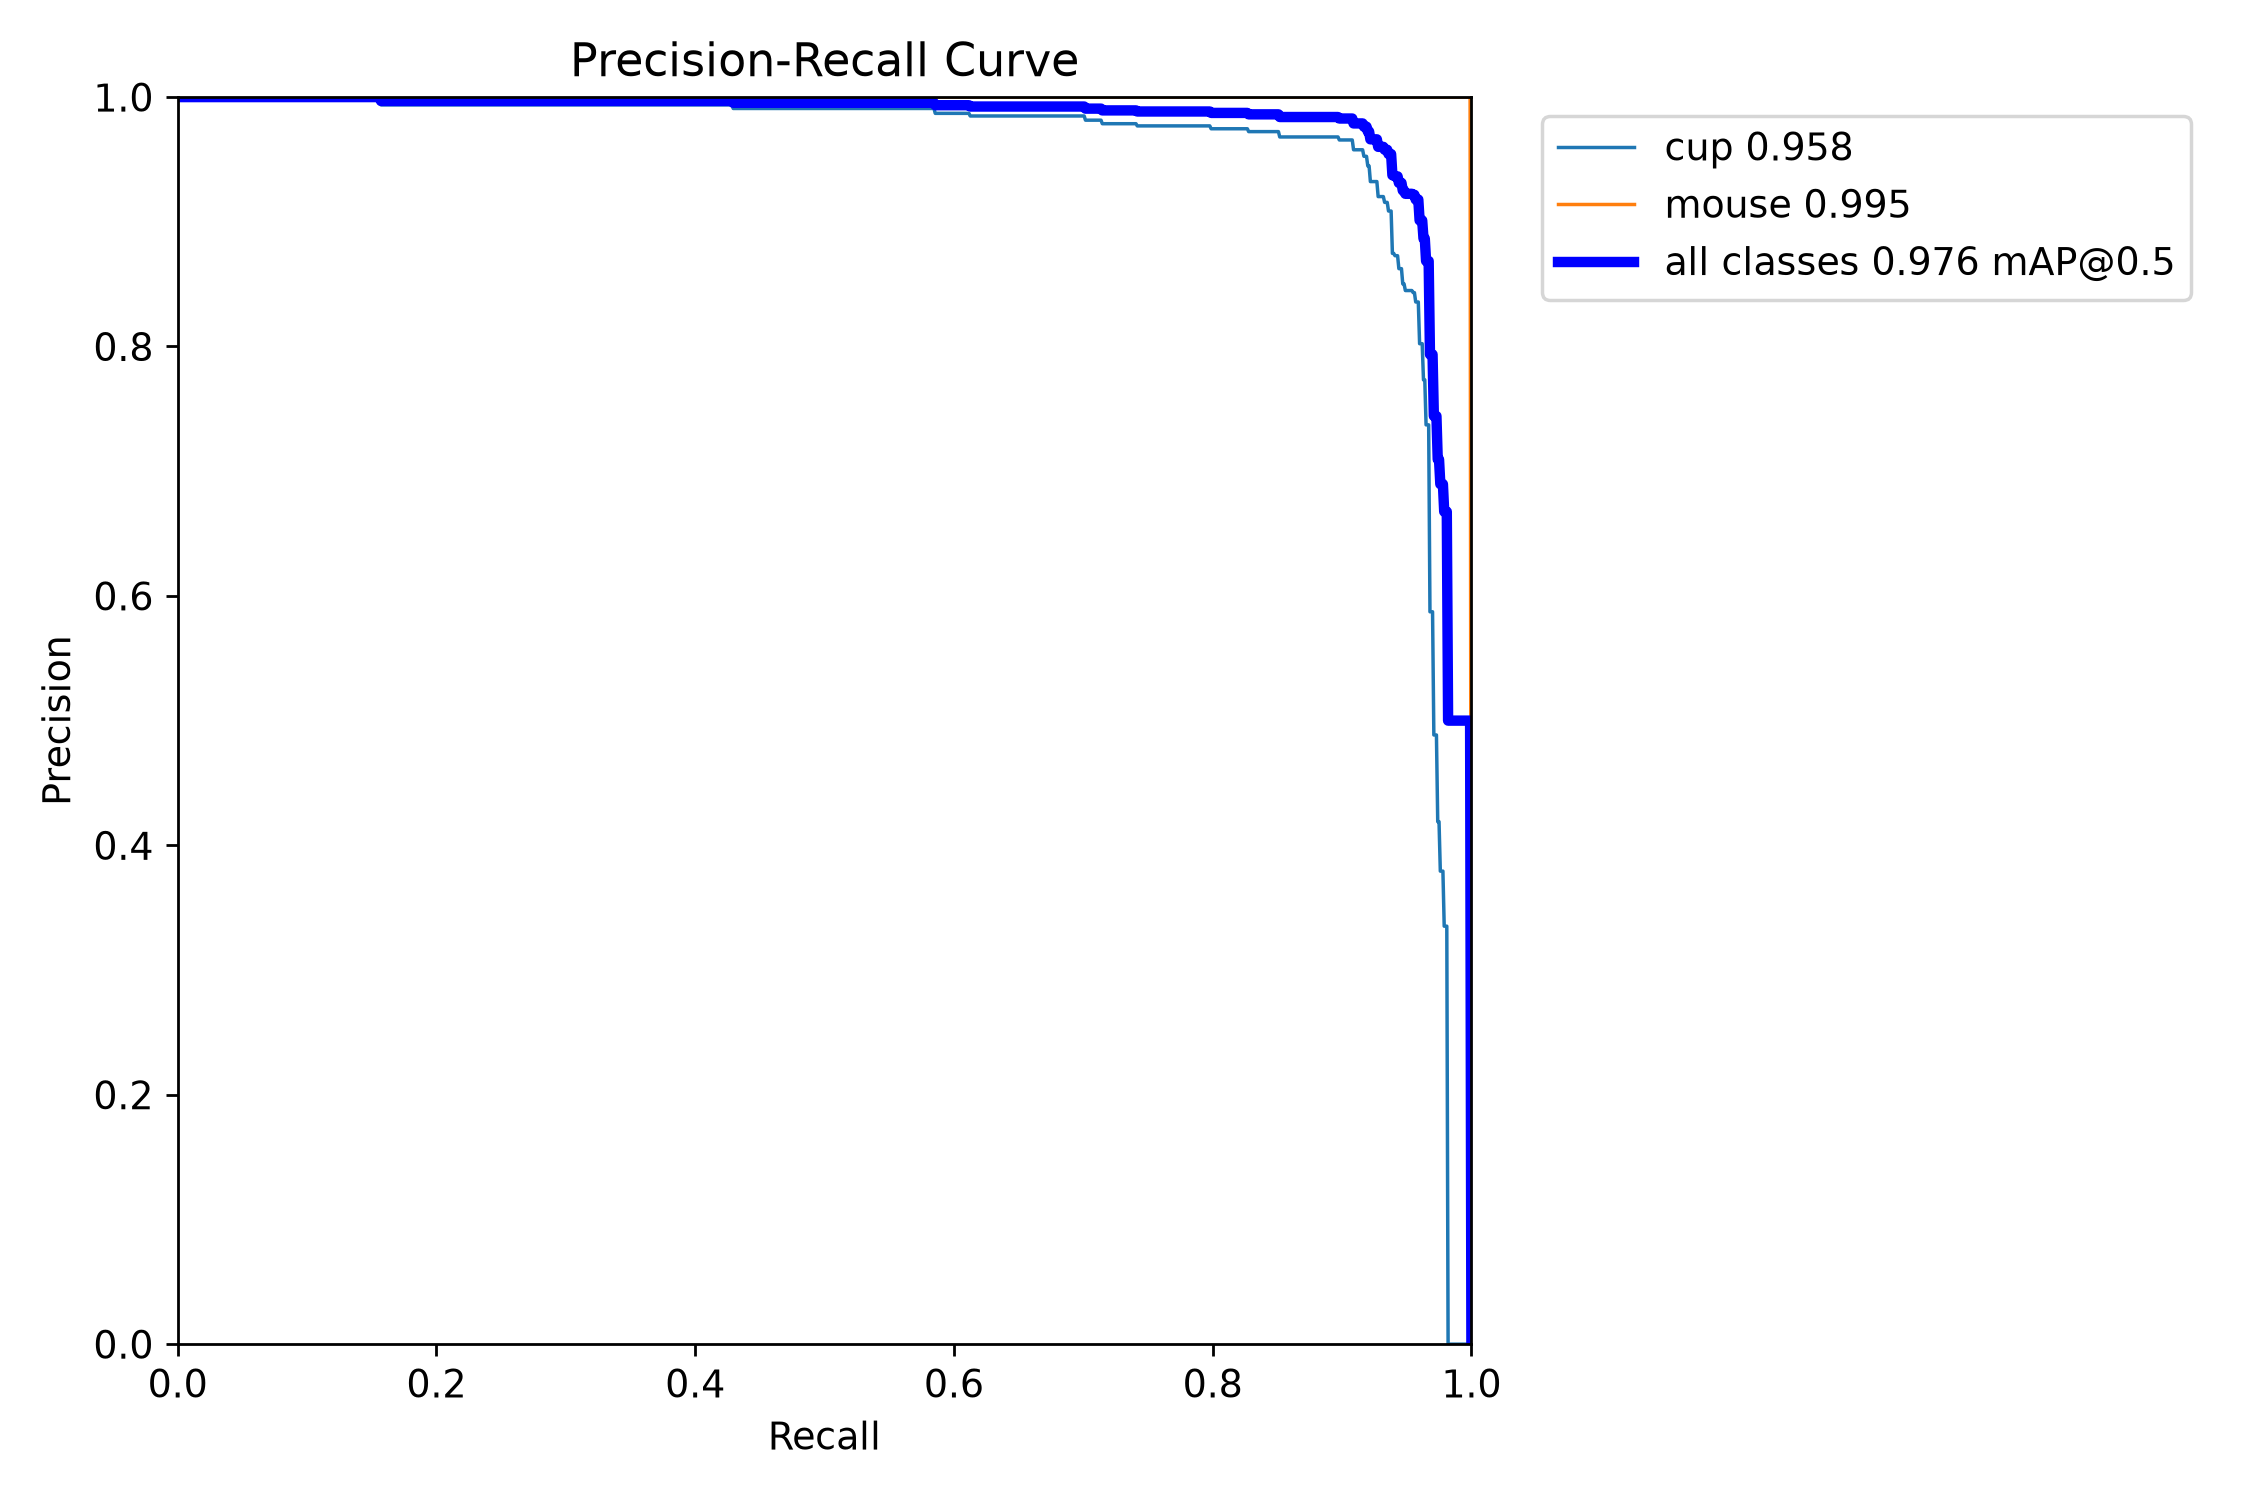
\includegraphics[width=\textwidth]{pr_curve.png}
    \caption{PR 曲线}
  \end{subfigure}
  \hfill
  \begin{subfigure}[b]{0.45\textwidth}
    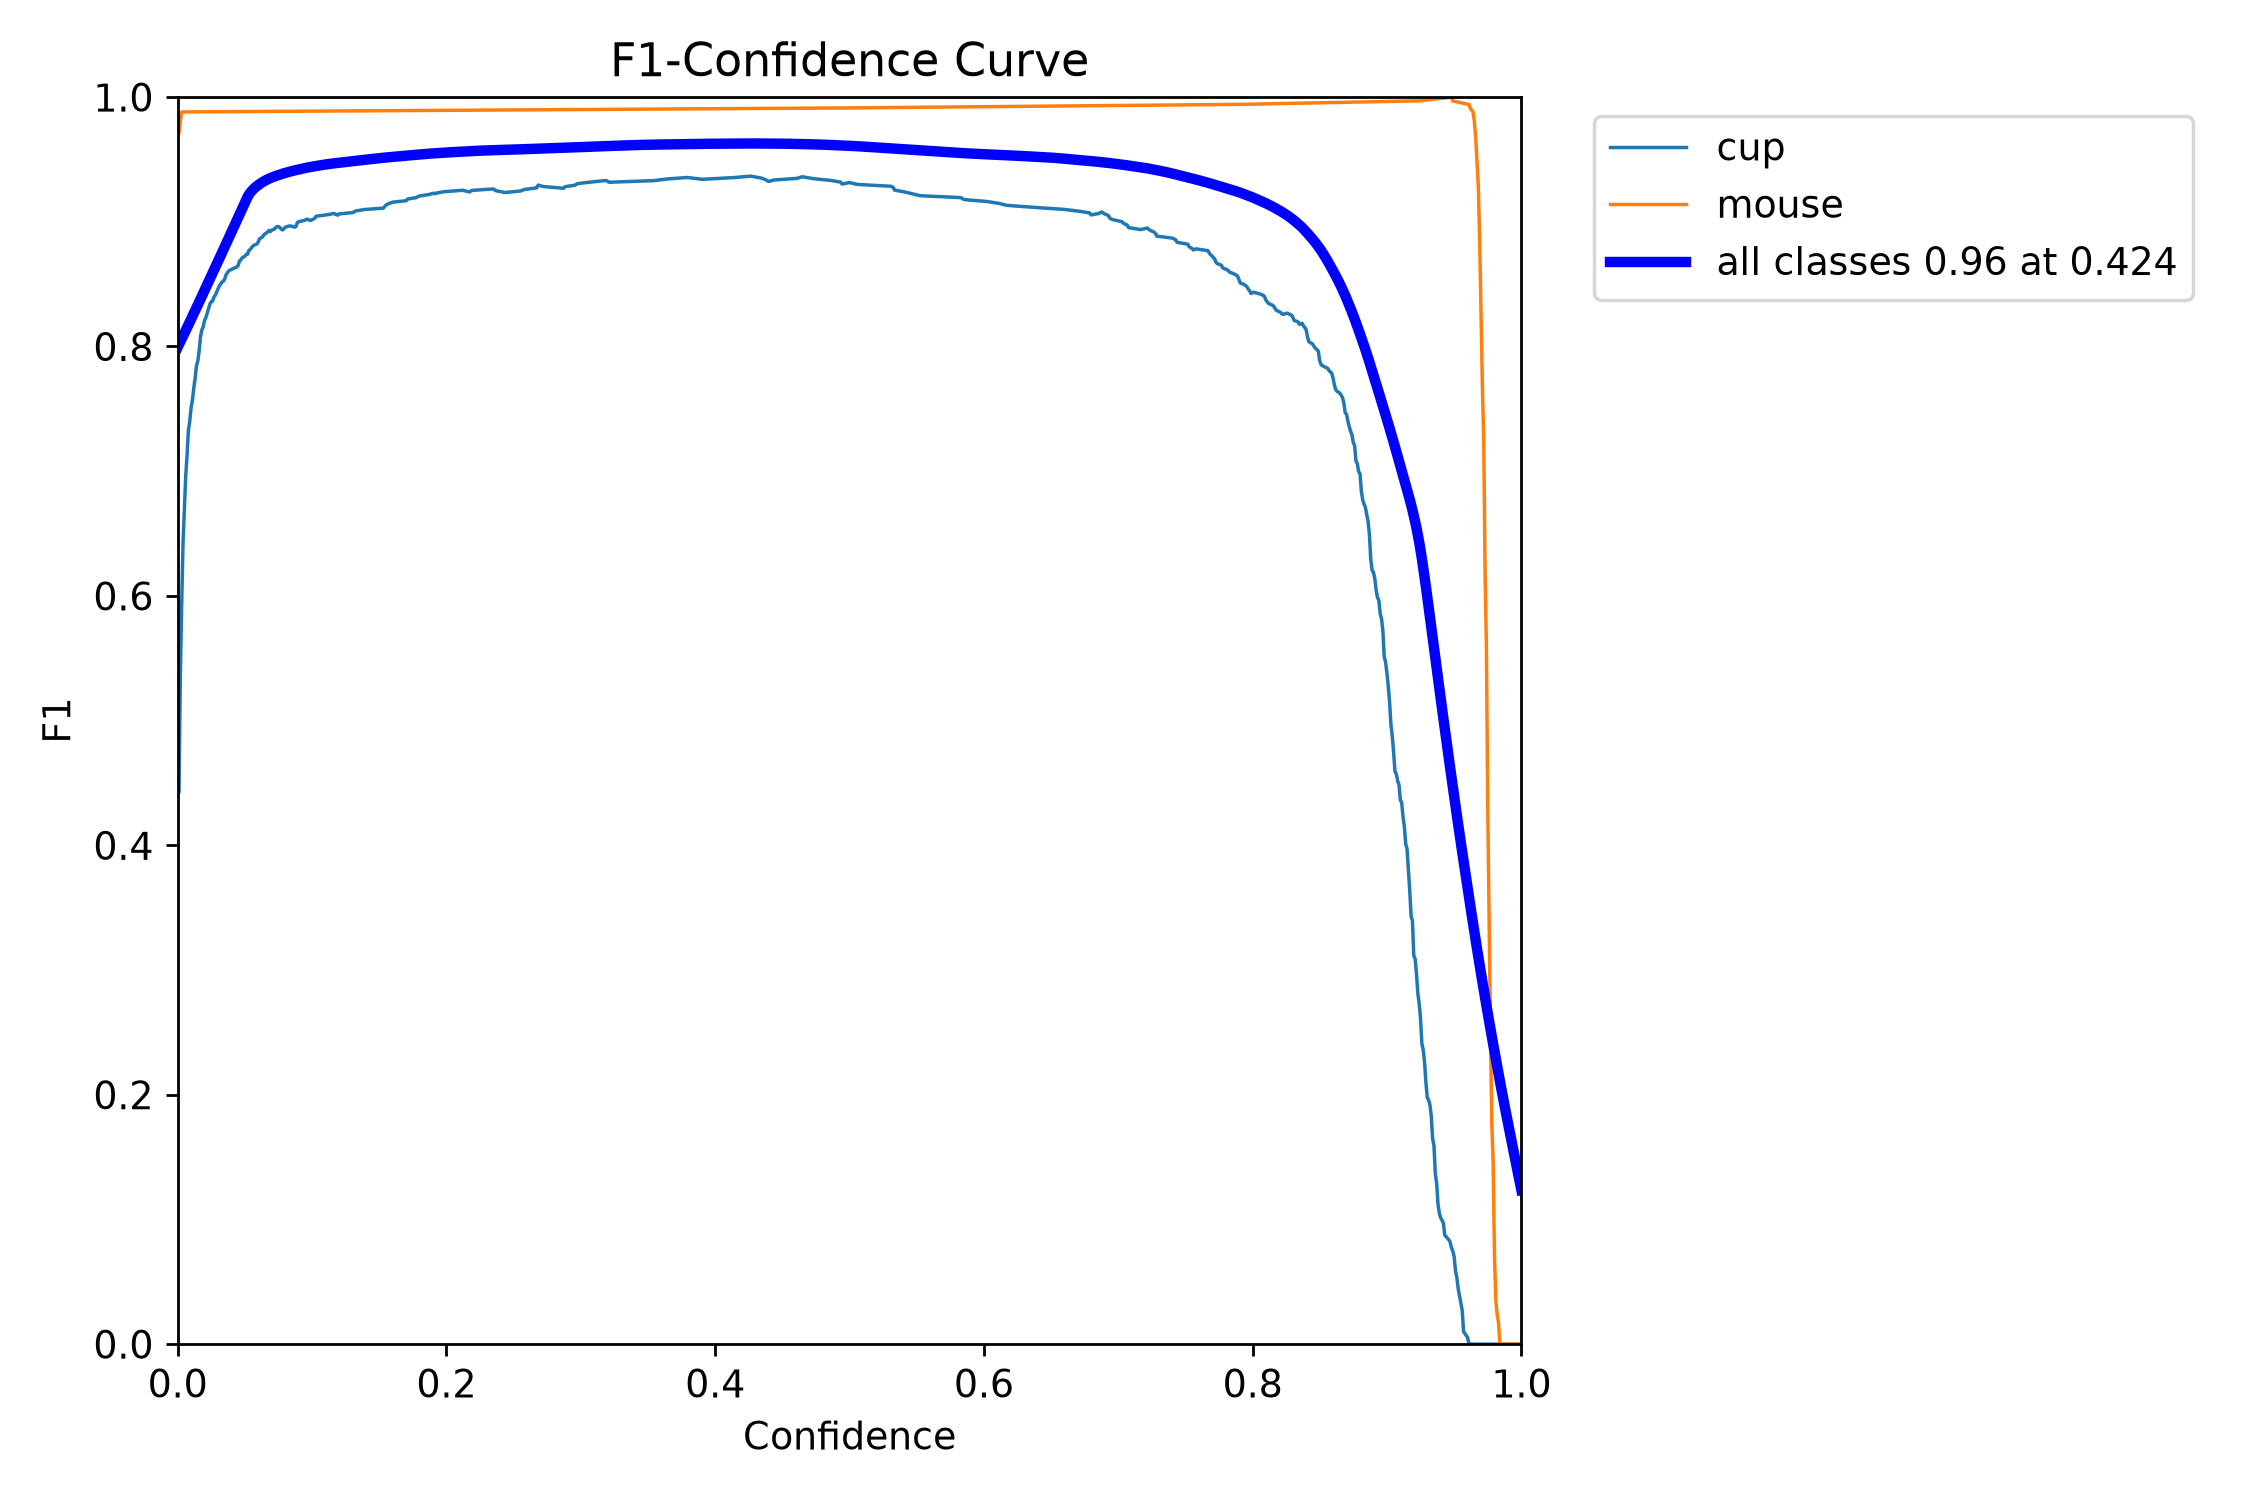
\includegraphics[width=\textwidth]{f1_curve.png}
    \caption{F1-Confidence 曲线}
  \end{subfigure}
  \caption{验证集 PR 与 F1 曲线}
\end{figure}

\begin{figure}[htbp]
  \centering
  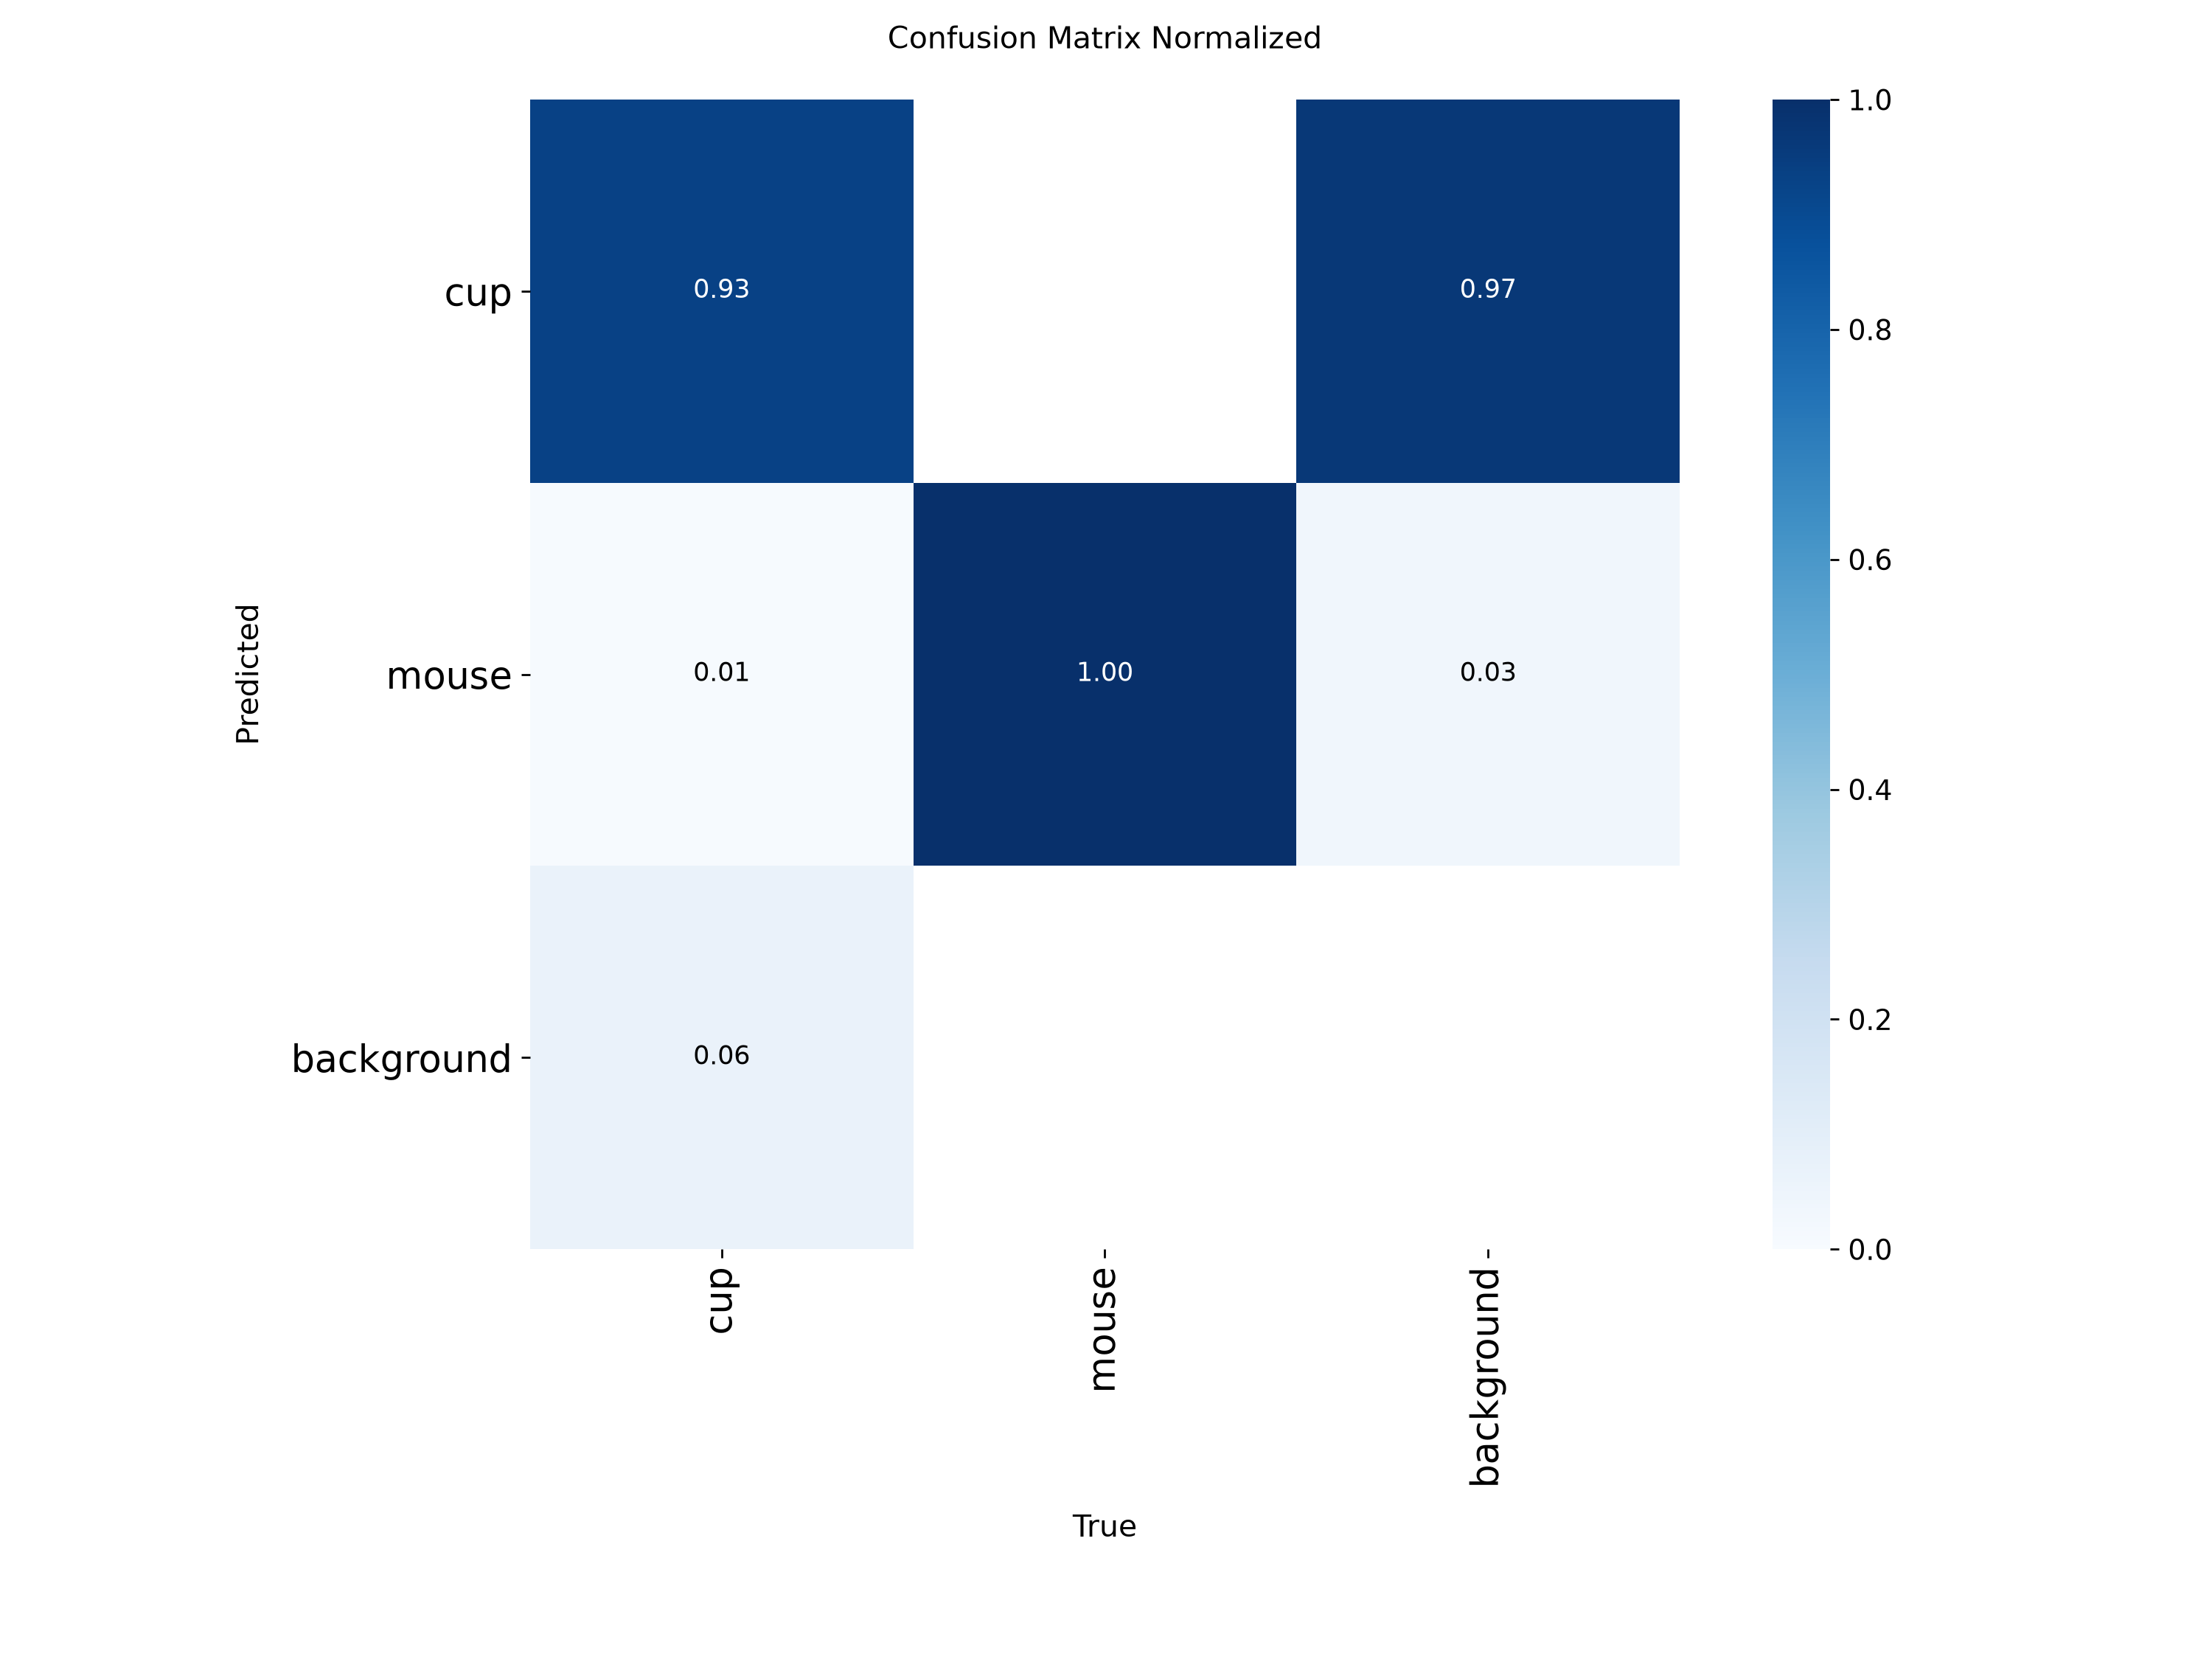
\includegraphics[width=0.55\textwidth,keepaspectratio]{confusion_matrix.png}
  \caption{验证集归一化混淆矩阵（右上：MOTA 指标，非重点）}
\end{figure}

\subsection{个人测试集结果}
%% 由 scripts/gen_report_assets.py 生成
\begin{table}[htbp]
\centering
\caption{个人测试集按类别准确率（验收要求整体 $\geq 80\%$）}
\begin{tabular}{l c c c c}
\toprule
类别 & 测试数 & 正确 & 正确率 & 平均置信度 \\
\midrule
cup & 10 & 10 & 100\% & 0.861 \\
mouse & 10 & 9 & 90\% & 0.871 \\
\midrule 总体 & 20 & 19 & 95\% & -- \\
\bottomrule
\end{tabular}
\end{table}

%% 混淆情况（行=真值，列=预测）
\begin{table}[htbp]
\centering
\caption{混淆矩阵（行：真值，列：预测，none=未检出）}
\begin{tabular}{l c c c}
\toprule
真值$\backslash$预测 & cup & mouse & none \\
\midrule
cup & 10 & 0 & 0 \\
mouse & 1 & 9 & 0 \\
\bottomrule
\end{tabular}
\end{table}


逐张结果见表 \ref{tab:test_results}，验证集预测示例见图。

%% 由 scripts/gen_report_assets.py 从 results/test_results.csv 自动生成，勿手改
\begin{longtable}{r l l l c c}
\caption{个人测试集逐张结果（20 张，10 cup + 10 mouse，阈值 conf=0.25）}\label{tab:test_results}\\
\toprule 编号 & 图片 & 真值 & 预测 & 置信度 & 正确 \\
\midrule \endhead
\bottomrule \endlastfoot
1 & \texttt{210c7479f15deb21a0b9003384c3f188.jpg} & cup & cup & 0.907 & \checkmark \\
2 & \texttt{3c735b9582257134e28f199c31a4374a.jpg} & cup & cup & 0.926 & \checkmark \\
3 & \texttt{7549e122789e0eec4f7b02a0c5c1f925.jpg} & cup & cup & 0.91 & \checkmark \\
4 & \texttt{7b0e09b9ce717549ff105ecdf719b56d.jpg} & cup & cup & 0.914 & \checkmark \\
5 & \texttt{7e6bf69bbda89c048b2172084f439238.jpg} & cup & cup & 0.865 & \checkmark \\
6 & \texttt{854c298a966e78777b85800c8b396094.jpg} & cup & cup & 0.857 & \checkmark \\
7 & \texttt{876f5820cd06c68558b507296e37de8a.jpg} & cup & cup & 0.892 & \checkmark \\
8 & \texttt{c27d20c6db65de8a7cd3ce8d0b72e6ad.jpg} & cup & cup & 0.736 & \checkmark \\
9 & \texttt{dc920cc1a19b41575c05270d52f54951.jpg} & cup & cup & 0.729 & \checkmark \\
10 & \texttt{f357eedb11b092c22a73f0119b357d2d.jpg} & cup & cup & 0.871 & \checkmark \\
11 & \texttt{531338c9c2eff75374d2e698d9af526f.jpg} & mouse & mouse & 0.968 & \checkmark \\
12 & \texttt{560c77473deb37dea04400586decbd79.jpg} & mouse & mouse & 0.975 & \checkmark \\
13 & \texttt{602fa7085b03a9f313173874ad2a437d.jpg} & mouse & mouse & 0.96 & \checkmark \\
14 & \texttt{638f2ca22261aff7caf032e2eb1bc30c.jpg} & mouse & mouse & 0.943 & \checkmark \\
15 & \texttt{a79a99a9584a0bb927167853bd0431b5.jpg} & mouse & cup & 0.499 & \ensuremath{\times} \\
16 & \texttt{abaf5e01a53905121de111580899f3b1.jpg} & mouse & mouse & 0.966 & \checkmark \\
17 & \texttt{aeef8b1c80a958aa6cb0a9f6b2d8bd60.jpg} & mouse & mouse & 0.522 & \checkmark \\
18 & \texttt{c0c80606c97bbb4511190f05cca36903.jpg} & mouse & mouse & 0.969 & \checkmark \\
19 & \texttt{f365468e77cd2d69d49190d35a690ac7.jpg} & mouse & mouse & 0.943 & \checkmark \\
20 & \texttt{f732c7623daf01820e5b46cf3d22bfd9.jpg} & mouse & mouse & 0.968 & \checkmark \\
\end{longtable}


\begin{figure}[htbp]
  \centering
  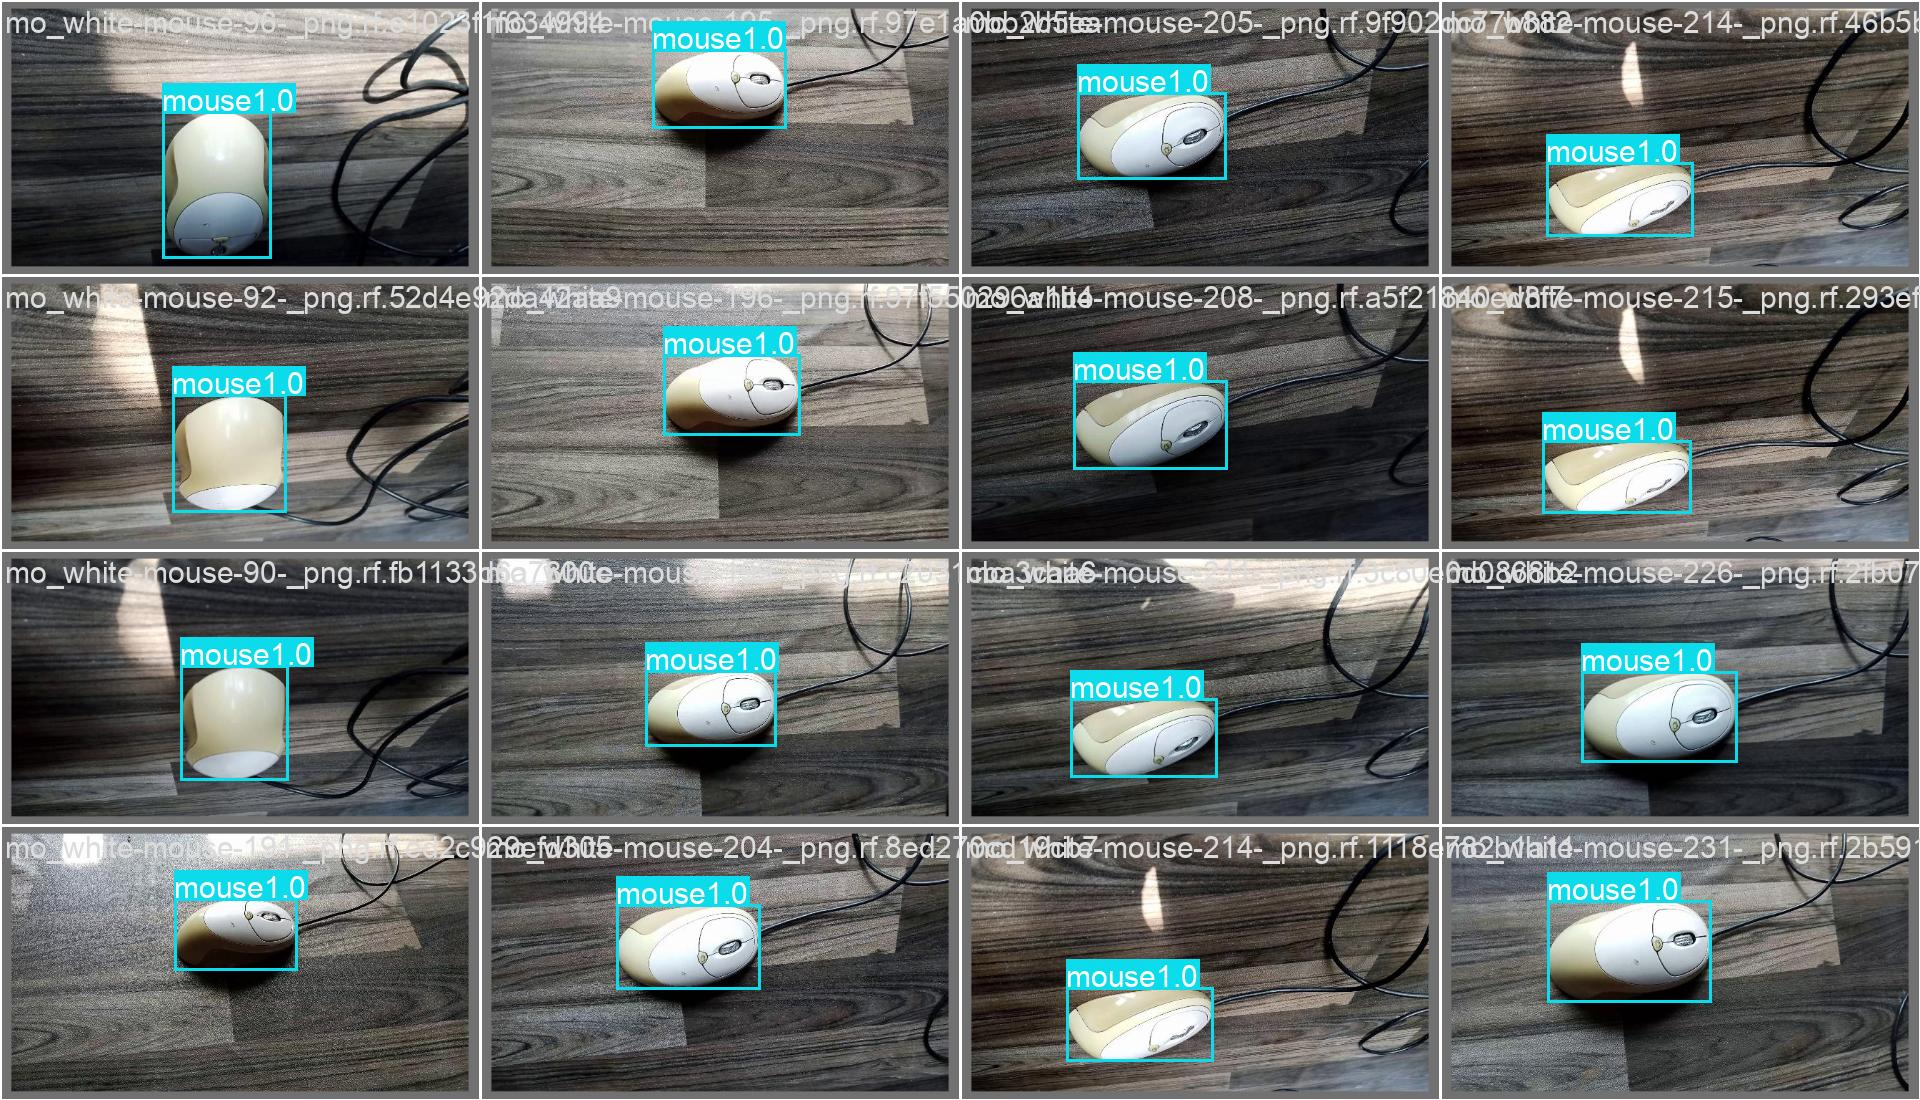
\includegraphics[width=0.9\textwidth,keepaspectratio]{val_pred.jpg}
  \caption{验证集预测示例（绿色框=cup，橙色框=mouse）}
\end{figure}

\subsection{典型错误案例分析}
个人测试集共 1 例错误：一张竖拍 960$\times$1280 的鼠标图片，目标紧贴画面上边缘、
部分出框，模型以较低置信度 \textbf{0.499} 误判为杯子，见图。

\begin{figure}[htbp]
  \centering
  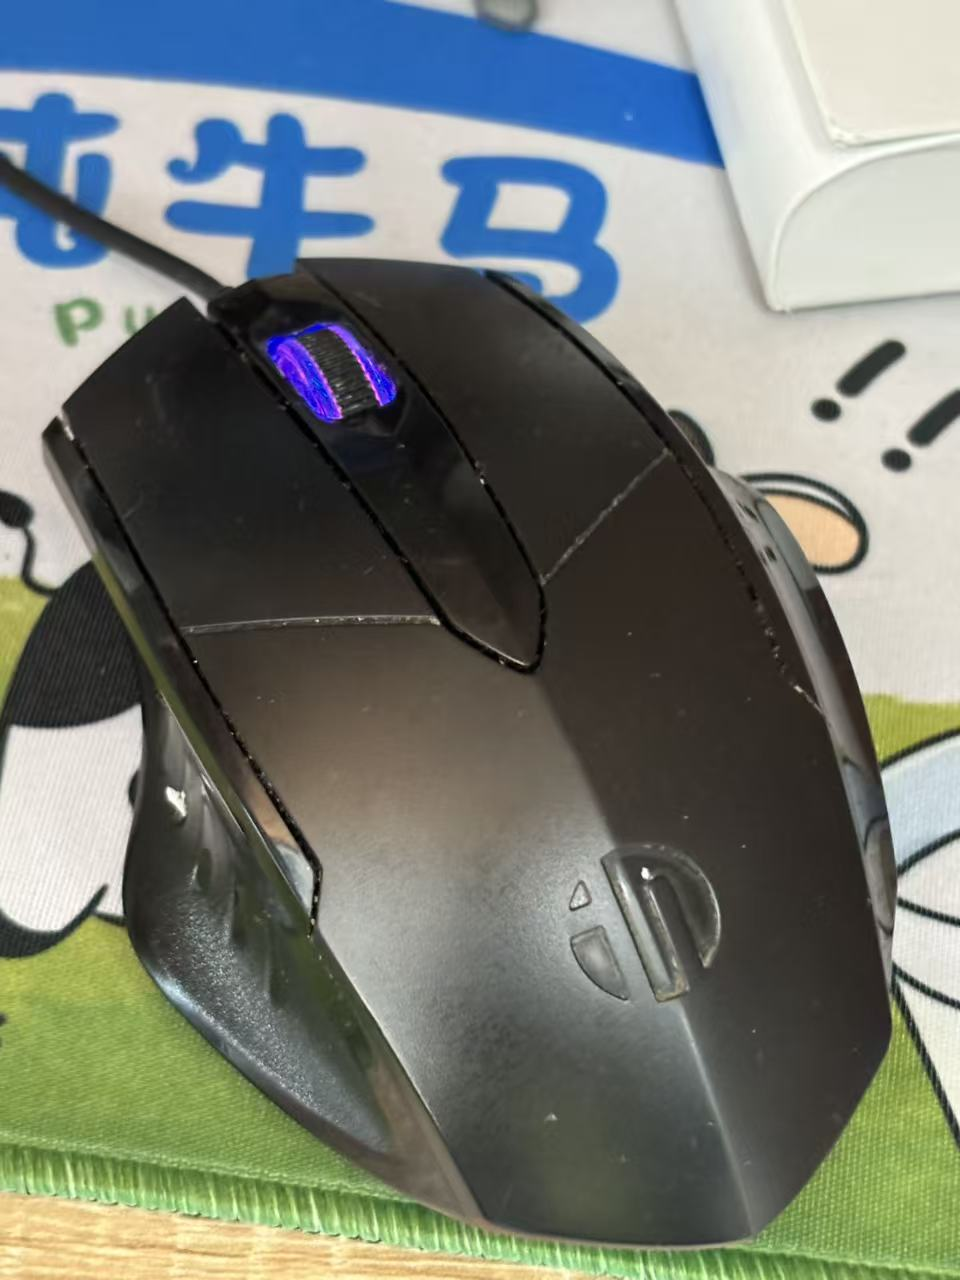
\includegraphics[width=0.35\textwidth,keepaspectratio]{error_case.jpg}
  \caption{错误案例：目标贴顶出框的鼠标被误判为杯子（conf 0.499）}
\end{figure}

\noindent 分析：该图目标只露出上半部分，与训练集中常见的完整鼠标形态差异较大，
且置信度仅 0.499（接近阈值 0.25 之上不高），属于极端姿态下的域外样本。
改进方向：\emph{①} 用 collect\_data.py 补充该姿态（贴边/出框/竖拍）的个人数据
参与训练；\emph{②} 提高置信度阈值或引入 NMS 后的目标完整性约束；\emph{③}
在报告期说明该案例已作为典型误差样例收录。

\subsection{结果讨论}
\begin{itemize}
  \item \textbf{类别不平衡的解决}：旧版合并数据鼠标标注缺失（0 标注）导致模型将
        鼠标全判为杯子；重构为 1500:1110 平衡数据后，鼠标准确率从 0\% 提升至 90\%。
  \item \textbf{领域差异}：公开数据训练的模型对个人桌面环境存在域差异，
        建议后续采集 100+ 张个人图片（含鼠标）补充训练，可进一步提升边缘情况鲁棒性。
\end{itemize}

\section{Jetson 部署与实时识别}
\subsection{总体流程}
\begin{figure}[htbp]
  \centering
  \begin{tikzpicture}[
      node distance=0.3cm, auto,
      box/.style={draw, rectangle, rounded corners, minimum height=1.1cm,
                  align=center, text width=2.9cm, font=\small},
      arrow/.style={-{Stealth}, thick},
    ]
    \node[box] (cam) {USB/CSI\\摄像头};
    \node[box, right=0.9cm of cam] (eng) {PyTorch FP16\\yolov8s@640 CUDA};
    \node[box, right=0.9cm of eng] (det) {实时识别程序\\绘制框+置信度+FPS};
    \node[box, right=0.9cm of det] (ros) {ROS2 节点\\发布 /detections};
    \draw[arrow] (cam) -- (eng);
    \draw[arrow] (eng) -- (det);
    \draw[arrow] (det) -- (ros);
  \end{tikzpicture}
  \caption{Jetson 端推理与发布流程}
\end{figure}

\subsection{FP16 加速推理}
将训练得到的 \texttt{best.pt} 加载到 Jetson 的 CUDA GPU 上，以 FP16 精度实时推理：
\begin{lstlisting}[style=code,language=bash]
python3 jetson/detect.py --model models/combined_best.pt --half
# SSH 无显示环境：加 --no-show --save-interval 3（自动存帧 + 打印 FPS）
\end{lstlisting}
FP16 CUDA 推理下 yolov8s@640 在 Orin NX 上实测 \textbf{24--25 FPS}，远超 5 FPS 的
验收下限。\footnote{本实验板子的 JetPack 镜像缺少 \texttt{libnvdla\_compiler.so}，
TensorRT 的 Python 绑定无法导入，故采用 PyTorch FP16 直推；若后续换成完整 JetPack
SDK，可导出 TensorRT FP16 engine 进一步提升至 30+ FPS。}且推理可在无显示器（SSH）
环境下以 \texttt{--no-show} 模式自动存帧并打印 FPS。

\subsection{演示视频与结果验证}
以 \texttt{--record} 录制 70 秒实时检测视频（640$\times$480，12.24 FPS 重封装为
真实速度），完整记录三类片段：杯子单独、鼠标单独、两者同框，帧上始终叠加
类别/置信度/检测框与 FPS 计数。录制使用新增的 \texttt{--duration} 参数，到点由
程序正常收尾，保证 MP4 文件完整：
\begin{lstlisting}[style=code,language=bash]
python3 jetson/detect.py --model models/combined_best.pt --half \
    --record results_video/demo_detect.mp4 --duration 70
# 校验（scripts/analyze_video.py 逐帧统计，脚本随仓库提交）
python3 scripts/analyze_video.py results/video/demo_detect.mp4
\end{lstlisting}
对录制视频逐帧校验：杯框出现 60 s、鼠框 60 s、两者同框 51 s、FPS 红字全程
70 s 均有叠加，双类均被稳定识别。演示视频见 \texttt{results/video/demo\_detect.mp4}，
其中一帧见图。

\begin{figure}[htbp]
  \centering
  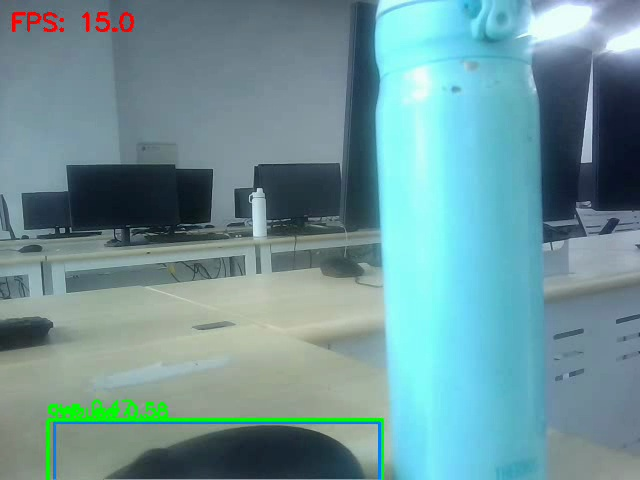
\includegraphics[width=0.62\textwidth,keepaspectratio]{demo_video_frame.jpg}
  \caption{演示视频第 55 s 帧：杯、鼠同时检出并实时叠加类别/置信度/检测框与 FPS}
\end{figure}

\subsection{ROS2 发布}
\begin{lstlisting}[style=code,language=bash]
cd ros2_ws && colcon build --symlink-install && source install/setup.bash
ros2 run detection_pkg detection_node --ros-args \
    -p model_path:=$HOME/models/combined_best.pt -p camera_index:=0 \
    -p device:=0 -p half:=true -p show:=false
# 另一终端订阅：
ros2 topic echo /detections
\end{lstlisting}
节点将每帧检测结果以 JSON 字符串发布到 \texttt{/detections} 话题，格式示例：
\begin{lstlisting}[style=code]
[{"class": "mouse", "confidence": 0.968,
  "bbox": [85.7, 133.6, 190.8, 232.3]}]
\end{lstlisting}

\section{结论与展望}
\subsection{结论}
\begin{itemize}
  \item 完成杯、鼠双类 YOLOv8 检测模型：验证集 mAP50 = 0.975；
  \item 个人测试集 20 张：cup 100\% / mouse 90\% / 总体 95\%，满足 $\geq 80\%$ 验收；
  \item Jetson Orin NX 上 FP16 CUDA 实时推理实测 24--25 FPS，满足 $\geq 5$ FPS，
        并实时显示类别/框/置信度；
  \item 检测结果经 ROS2 以 /detections 话题实时发布，可被其他节点消费；
  \item 全部代码、数据与结果以增量提交方式托管于个人 GitHub。
\end{itemize}
\subsection{展望}
\begin{itemize}
  \item 补充更多个人采集数据（尤其边缘/遮挡/极端姿态）进一步缩小域差异；
  \item 尝试 INT8 量化与更轻量骨干（yolov8n），提升边缘设备上的吞吐与功耗表现；
  \item 扩展类别数（键盘、手机等）并引入目标跟踪，支撑更复杂的桌面理解应用。
\end{itemize}

% ============================== 参考文献 ==============================
\begin{thebibliography}{9}
  \bibitem{ultralytics} Jocher G, Chaurasia A, Qiu J. Ultralytics YOLOv8
    [CP/OL]. (2023). https://github.com/ultralytics/ultralytics.
  \bibitem{yolo_review} Terven J, C'ordova-Esparza D M, Romero-Gonz'alez J A.
    A Comprehensive Review of YOLO Architectures in Computer Vision
    [J]. Journal of Big Data, 2023, 10(1): 29.
  \bibitem{tensorrt} NVIDIA. TensorRT: High Performance Deep Learning Inference
    [CP/OL]. https://developer.nvidia.com/tensorrt.
  \bibitem{roboflow} Roboflow. Computer-Mouse Dataset (v2, CC BY 4.0)
    [DB/OL]. https://universe.roboflow.com/machine-learning-chipg/computer-mouse-tqzgh/dataset/2.
  \bibitem{roboflow_cup} Roboflow. Cup Detection (v3, CC BY 4.0) [DB/OL].
    https://universe.roboflow.com/my-workspace-7j2fi/cup-detection-w8kfb/dataset/3.
  \bibitem{coco} Lin T Y, Maire M, Belongie S, et al. Microsoft COCO: Common
    Objects in Context [C]//ECCV. 2014: 740--755.
\end{thebibliography}

% ============================== 附录 ==============================
\appendix
\section{Git 提交记录（增量提交，符合验收要求）}
\VerbatimInput{gitlog.txt}

\section{复现方法}
训练与评估关键命令：
\begin{lstlisting}[style=code,language=bash]
# 1. 构建平衡数据集（1500 cup : 1110 mouse）
python3 scripts/build_combined_dataset.py --cup-src public_data/combined \
    --mouse-src public_data/mouse_rf_653/extracted \
    --out public_data/balanced --max-cups 1500 --val-split 0.15

# 2. 训练（本地 MPS 或云端 CUDA 均可，自动检测）
python3 scripts/train_combined.py

# 3. 个人测试集评估（输出 results/test_results.csv 与错误案例）
python3 scripts/evaluate.py --model runs/detect/combined_model_v3/weights/best.pt \
    --test-root test_images --conf 0.25

# 4. 生成报告图表素材（本模板插图/表格的来源）
python3 scripts/gen_report_assets.py
\end{lstlisting}

\section{目录结构说明}
\begin{lstlisting}[style=code]
object_detection_lab/
├── public_data/balanced/       # 平衡合并数据集（train/val + data_balanced.yaml）
├── personal_data/              # 个人采集训练数据（可选补充）
├── test_images/{cup,mouse}     # 个人测试集 20 张（不参与训练）
├── scripts/                    # 数据构建/训练/评估/导出/打包脚本
├── jetson/detect.py            # Jetson 实时识别程序
├── ros2_ws/src/detection_pkg/  # ROS2 发布节点
├── runs/detect/combined_model_v3/  # 训练权重与图表
└── report/                     # 本报告模板与素材
\end{lstlisting}

\end{document}
